Why should I learn a new method if I already got \textit{linear regression} and \textit{logistic regression} (for classification). We saw that, in order to fit our model to the data, we can add more variables or increase the order of the polynomial but to achieve that we gotta do a lot of try/error. Wouldn't it be nice to have a method that self-learns the shape of the decision boundary based on all combinations of input data? or do the same for the shape of the polynomial regression ? That's where \textbf{neural networks} are for !!. Generally, we use neural networks to solve classification problems.

\subsection{Representation and Concepts}

The representation for neural networks is:

\begin{align}
	\begin{bmatrix}
		x_0 \\
		x_1 \\
		x_2 \\
	\end{bmatrix}
	\rightarrow
	\begin{bmatrix}
		a_1^{(2)} \\
		a_2^{(2)} \\
	\end{bmatrix}
	\rightarrow
	h_{\theta}(x) \label{neural-network-rep}
\end{align}

The first vector ($x_j$) is called \textbf{input layer} ($x_i$), it's length will be $n + 1$ ($n$ is the number of features, we add 1 because of the unit bias $x_0$). 

The last item is the \textbf{output layer}($h_{\theta}(x)$) and can be a vector too, it represents the final answer which is the prediction (whether $0$ or $1$).

The layer(s) between \textit{input} and \textit{output} layers are called \textbf{hidden layer}. Each node in the layer is called \textbf{activation unit} that is a sigmoid function.

The relationship between layers is a matrix of weights ($\Theta^{(j)}$). Since it's a relationship it has to map all the combinations between the layers $j$ and $j + 1$, but we only include the unit bias of the layer j (add one to the number of the layer $j$), the bias unit is always 1 (because it will be directly multiplied by the activation unit). So it's length will be:

\begin{align}
\Big[\text{\# of units of layer } (j + 1)\Big] \times \Big[1 + \text{\# of units of layer } (j)\Big] \label{weight-matrix-size}
\end{align}

\newpage
\noindent In summary, these are the representations:

\begin{align*}
	& s_j = \text{number of units of layer } j \\
	& a^{(j)}_i = \text{"activation" of unit } i \text{ in the layer } j \\
	& \Theta^{(j)} = \text{matrix of weights controlling function mapping from layer } j \text{ to layer } j + 1 \\ 
\end{align*}

\noindent Another way to present the neural network would be:
\begin{figure}[h]
    \centering
    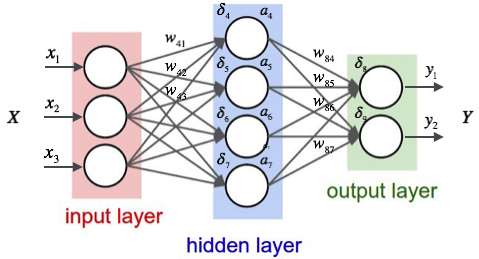
\includegraphics[width=1\textwidth]{neural-network-concept}
    \caption{Neural Network}
    \label{fig:neural-network-concept}
\end{figure}

\noindent In the representation \eqref{neural-network-rep} the values for the activation units are:

\begin{align*}
	a^{(2)}_1 = g(\Theta^{(1)}_{10}x_0 + \Theta^{(1)}_{11}x_1 + \Theta^{(1)}_{12}x_2) \\
	a^{(2)}_2 = g(\Theta^{(1)}_{20}x_0 + \Theta^{(1)}_{21}x_1 + \Theta^{(1)}_{22}x_2) \\
\end{align*}

\noindent And the value of the hypotheses function will be:

$$h_{\Theta}(x) = g(\Theta^{(2)}_{10}a^{(2)}_0 + \Theta^{(2)}_{11}a^{(2)}_1 + \Theta^{(2)}_{12}a^{(2)}_2) = \Big\{^1_0 $$

\noindent This is saying that we compute our activation nodes by using a $2 \times 3$ (formula in \ref{weight-matrix-size}) matrix of parameters. We apply each row of the parameters to our inputs to obtain the value for one activation node. Our hypothesis output is the logistic function applied to the sum of the values of our activation nodes, which have been multiplied by yet another parameter matrix $\Theta^{(2)}$ containing the weights for our second layer of nodes. Each layer gets its own matrix of weights, $\Theta^{(j)}$.

We are going to introduce a new variable $z_k^{(j)}$ that encompasses the parameters inside our $g$ function. In our previous example if we replaced by the variable z for all the parameters we would get:

\begin{align*}
	a^{(2)}_1 = g(z^{(2)}_1) \\
	a^{(2)}_2 = g(z^{(2)}_2) \\
\end{align*}

\noindent In other words, for layer $j=2$ and node $k$, the variable $z$ will be:

$$z^{(2)}_k = \Theta^{(1)}_{k,0}x_0 + \Theta^{(1)}_{k,1}x_1 + \hdots + \Theta^{(1)}_{k,2}x_2$$


\subsection{Intuition - (what does a neural network actually learns)}
A simple example of applying neural networks is by predicting $x_1 AND x_2$, which is the logical 'and' operator and is only true if both $x_1$ and $x_2$ are $1$.

\noindent The graph of our functions will look like:

\begin{align}
	\begin{bmatrix}
		x_0 \\
		x_1 \\
		x_2 \\
	\end{bmatrix}
	\rightarrow
	\begin{bmatrix}
		g(z^{(2)}) \\
	\end{bmatrix}
	\rightarrow
	h_{\Theta}(x) \label{neural-network-rep}
\end{align}

\noindent (Remember that x0 is our bias variable and is always 1).

\noindent Let's set our first theta matrix as:

$$\Theta^{(1)} = \Big[ -30 \qquad 20 \qquad 20\Big]$$

This will cause the output of our hypothesis to only be positive if both $x_1$ and $x_2$ are $1$. In other words:

\begin{align*}
	h_{\Theta}(x) = g(-30 + 20x_1 + 20x_2) \\
	\\
	x_1 = 0 \text{ and } x_2 = 0 \text{ then } g(-30) \approx 0 \\
	x_1 = 0 \text{ and } x_2 = 1 \text{ then } g(-10) \approx 0 \\
	x_1 = 1 \text{ and } x_2 = 0 \text{ then } g(-10) \approx 0 \\
	x_1 = 1 \text{ and } x_2 = 1 \text{ then } g(10) \approx 1 \\
\end{align*}

So we have constructed one of the fundamental operations in computers by using a small neural network rather than using an actual AND gate. Neural networks can also be used to simulate all the other logical gates.

For example, let's create a made-up gate: XNOR.

The $\Theta^{(1)}$ matrices for AND, NOR, and OR are:

\begin{align*}
	& AND: \\
	& \quad \Theta^{(1)} = \Big[ -30 \quad 20 \quad 20\Big] \\
	& NOR: \\
	& \quad \Theta^{(1)} = \Big[ 10 \quad -20 \quad -20\Big] \\
	& OR: \\
	& \quad \Theta^{(1)} = \Big[ -10 \quad 20 \quad 20\Big] \\
\end{align*}

We can combine these to get the XNOR logical operator (which gives $1$ if $x_1$ and $x_2$ are both $0$ or both $1$).


\begin{align}
	\begin{bmatrix}
		x_0 \\
		x_1 \\
		x_2 \\
	\end{bmatrix}
	\rightarrow
	\begin{bmatrix}
		a_1^{(2)} \\
		a_2^{(2)} \\
	\end{bmatrix}
	\rightarrow
	\begin{bmatrix}
		a^{(3)} \\
	\end{bmatrix}
	\rightarrow
	h_{\theta}(x)
\end{align}

For the transition between the first and second layer, we'll use a $\Theta^{(1)}$ matrix that combines the values for AND and NOR:

$$\Theta^{(1)} = \begin{bmatrix}
	-30 \quad 20 \quad 20 \\
	10 \quad -20 \quad -20 \\
\end{bmatrix}$$

For the transition between the second and third layer, we'll use a $\Theta^{(2)}$ matrix that uses the value for OR:

$$\Theta^{(1)} = \begin{bmatrix}
	-10 \quad 20 \quad 20 \\
\end{bmatrix}$$

Let's write out the values for all our nodes

\begin{align*}
	a^{(2)} = g(\Theta^{(1)} \cdot x) \\
	a^{(3)} = g(\Theta^{(2)} \cdot a^{(2)}) \\
	h_{\Theta}(x) = a^{(3)} \\
\end{align*}

And there we have the XNOR operator using a hidden layer with two nodes! The following summarizes the above algorithm:

\begin{figure}[h]
    \centering
    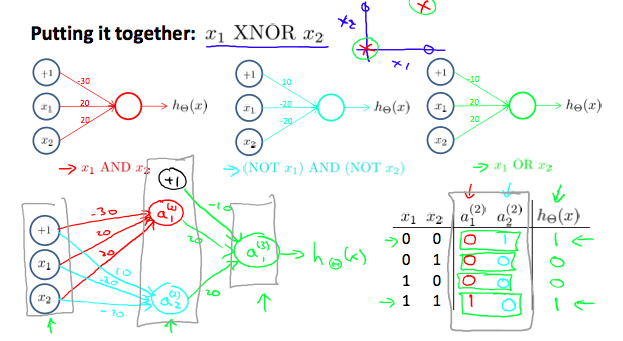
\includegraphics[width=1\textwidth]{neural-network-xnor}
    \caption{Neural Network $x_1 \text{ XNOR } x_2$}
    \label{fig:neural-network-xnor}
\end{figure}

\newpage
\subsection{Multiclass Classification}
To classify data into multiple classes, the output of the neural network will be a vector that has the length of the number of classes ($K$). Something like this:

\begin{align}
	\begin{bmatrix}
		x_0 \\
		x_1 \\
		x_2 \\
		\vdots \\
		x_n \\
	\end{bmatrix}
	\rightarrow
	\begin{bmatrix}
		a_0^{(2)} \\
		a_1^{(2)} \\
		a_2^{(2)} \\
		\vdots \\
	\end{bmatrix}
	\rightarrow
	\begin{bmatrix}
		a_0^{(3)} \\
		a_1^{(3)} \\
		a_2^{(3)} \\
		\vdots \\
	\end{bmatrix}
	\rightarrow
		\hdots
	\rightarrow
	\begin{bmatrix}
		h_{\Theta}(x)_1 \\
		h_{\Theta}(x)_2 \\
		h_{\Theta}(x)_3 \\
		h_{\Theta}(x)_4 \\
	\end{bmatrix}
\end{align}

\subsection{Cost function}

To understand all of the notations in the formula, we define a few variables:

\begin{enumerate}[label=\textbullet]
	\item $L$ = total number of layers in the network
	\item $s_l$ = number of units (not counting bias unit) in layer $l$
	\item $K$ = number of output units/classes
\end{enumerate}

Recall that in neural networks, we may have many output nodes. We denote $h_{\Theta}(x)_k$ as being a hypothesis that results in the $k^{th}$ th output. Our cost function for neural networks is going to be a generalization of the one we used for logistic regression showed in formula (\ref{logistic-regression}):

\begin{align*}
	J(\Theta) = - \frac{1}{m} \sum^m_{i=1}\sum^K_{k=1}\Bigg[ y^{(i)}_k log((h_{\theta}(x^{(i)}))_k) + (1 - y^{(i)}_k) log(1 - (h_{\theta}(x^{(i)}))_k) \Bigg] + \\
	\frac{\lambda}{2m}\sum^{L-1}_{l=1}\sum^{s_l}_{i=1}\sum^{s_{l+1}}_{j=1}(\Theta^{(l)})^2_{i,j}
\end{align*}

We have added a few nested summations to account for our multiple output nodes. In the first part of the equation, before the square brackets, we have an additional nested summation that loops through the number of output nodes.

In the regularization part, after the square brackets, we must account for multiple theta matrices. The number of columns in our current theta matrix is equal to the number of nodes in our current layer (including the bias unit). The number of rows in our current theta matrix is equal to the number of nodes in the next layer (excluding the bias unit). As before with logistic regression, we square every term.

\subsection{How to obtain $\Theta^{(l)}$}